% !TEX TS-program = xelatex
% !TEX encoding = UTF-8 Unicode
% !Mode:: "TeX:UTF-8"

\documentclass{resume}
\usepackage{tabu}
\usepackage{multirow}
\usepackage{progressbar}
\usepackage{zh_CN-Adobefonts_external} % Simplified Chinese Support using external fonts (./fonts/zh_CN-Adobe/)
% \usepackage{NotoSansSC_external}
% \usepackage{NotoSerifCJKsc_external}
% \usepackage{zh_CN-Adobefonts_internal} % Simplified Chinese Support using system fonts
\usepackage{linespacing_fix} % disable extra space before next section
\usepackage{cite}

\begin{document}
\pagenumbering{gobble} % suppress displaying page number

\Large{
  \begin{tabu}{ c l }
    \multirow{4}{0.9in}{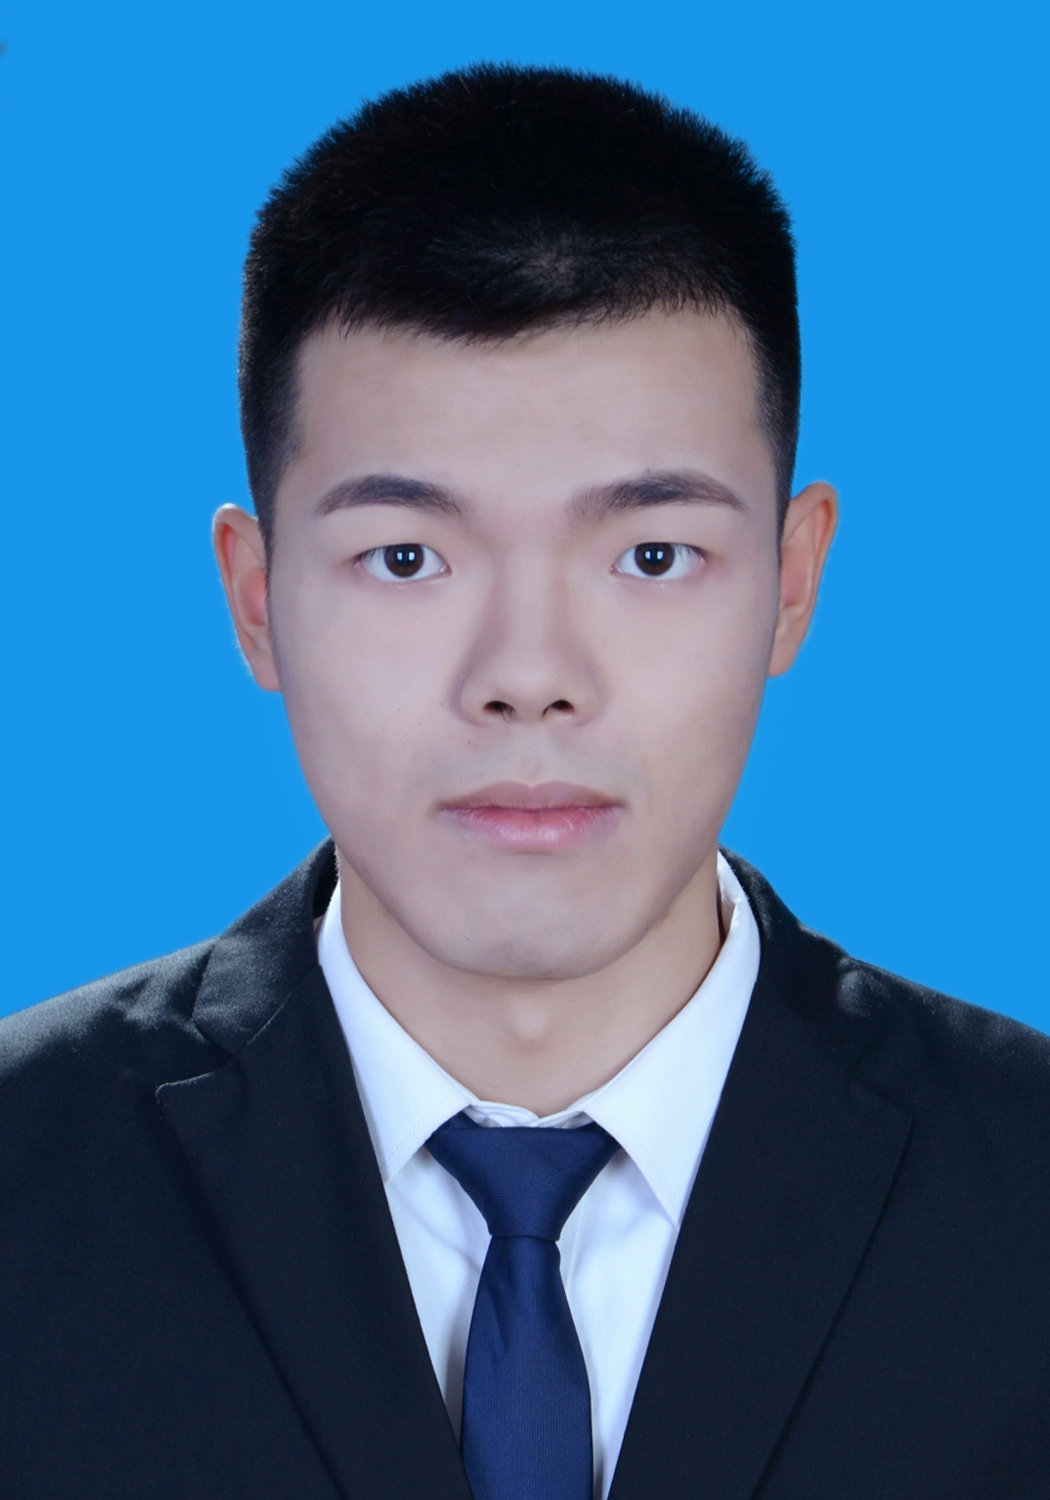
\includegraphics[width=0.7in]{photo.jpg}} & \scshape{李典源} \\
    & \phone{(+86) 156-597-72771} \\
    & \email{maybeldy@foxmail.com} \\
    & \github[github.com/lidotcircle]{https://github.com/lidotcircle} 
  \end{tabu}
}
\normalsize
\vskip 1ex

%\name{李典源}
%\basicInfo{
%  \email{maybeldy@foxmail.com} \textperiodcentered\ 
%  \phone{(+86) 156-59-772771} \textperiodcentered\ 
%}
 
\section{\faGraduationCap\  教育背景}
\datedsubsection{\textbf{福州大学}, \quad 福州}{2020年9月 -- 至今}
\textit{在读硕士研究生}\ 电子信息(计算机技术), 预计 2023 年 6 月毕业
\datedsubsection{\textbf{福州大学},\quad 福州}{2015年9月 -- 2019年6月}
\textit{学士}\ 土木工程


\section{\faUsers\ 实习/项目经历}
\datedsubsection{\textbf{网龙网络有限公司}, \quad 福州}{2021年8月 -- 2022年1月}
\role{实习}{游戏安全程序员}
\begin{onehalfspacing}
\begin{itemize}
  \item 主要进行游戏外挂样本分析、特征码提取
  \item 一些样本分析软件的开发(反反调试、代码注入)
\end{itemize}
\end{onehalfspacing}

\datedsubsection{\textbf{C99编译器}}{2022年1月 -- 至今}
\proj{个人项目}{C/C++}{https://github.com/lidotcircle/dcparse}
\begin{onehalfspacing}
\begin{itemize}
  \item 实现基本的正则表达式, 主要为了实现不匹配的字符串可以不需要全部输入就可判定为不匹配 
  \item 实现 Tokenizer 和 Parser Generator 进行解析C99语法
  \item 利用以上工具实现一个简易的 C-like 计算器
  \item 根据C99标准实现C99的Parser和初步的语法检查, 代码生成部分还未实现
\end{itemize}
\end{onehalfspacing}

\datedsubsection{\textbf{网盘}}{2019年3月 -- 至今}
\proj{个人项目}{Typescript, Angular, Express.js, typeorm, Docker}{https://github.com/lidotcircle/webdisk}
\begin{onehalfspacing}
\begin{itemize}
  \item 基于Web页面进行文件管理, 包括基本的文件管理操作、上传、下载、预览以及分享等功能, 并且支持多种后端的储存方式(硬盘、OSS, WebDAV)
  \item 使用ToastUI Editor集成了Markdown笔记功能
  \item 实现数据图表功能, 主要用于保存深度学习训练数据、结果, 可以作为tensorboard的替代品
\end{itemize}
\end{onehalfspacing}

% \datedsubsection{\textbf{Socks5代理}}{2019年4月 -- 至今}
% \proj{个人项目}{C/C++}{https://github.com/lidotcircle/hula}
% \begin{onehalfspacing}
% \begin{itemize}
%   \item 包含服务端和客户端的Socks5代理, 客户端和服务端之间通信使用TLS加密。并且复用TLS链接, 减少TLS握手的开销
% \end{itemize}
% \end{onehalfspacing}

\datedsubsection{\textbf{ScyllaMonitor}}{2021年11月 -- 至今}
\proj{个人项目}{C/C++, Dear ImGUI}{https://github.com/lidotcircle/ScyllaHide}
\begin{onehalfspacing}
\begin{itemize}
  \item 从ScyllaHide fork进行修改的反反调试、代码注入工具, 使用Dear ImGUI实现图形界面
  \item 利用inline hook实现代码注入功能, 支持32位和64位的程序
\end{itemize}
\end{onehalfspacing}

\section{\faCogs\ IT 技能}
% increase linespacing [parsep=0.5ex]
\begin{itemize}[parsep=0.5ex]
  \item 编程语言: C/C++ == Typescript > Java == Python
  \item 前端框架: Angular
  \item 后端开发: Node.js、Spring Boot
  \item 平台: Linux
  \item 开发工具: Git, Docker
  \item 深度学习: 基于对抗生成网络的图像翻译技术
\end{itemize}

% \section{\faArrowCircleRight\ 自我评价}
% 做事耐心, 喜欢学习新技术和新知识, 热爱编程

\section{\faInfo\ 其他}
% increase linespacing [parsep=0.5ex]
\begin{itemize}[parsep=0.5ex]
  \item 语言: 英语 (CET-6)
\end{itemize}

%% Reference
%\newpage
%\bibliographystyle{IEEETran}
%\bibliography{mycite}
\end{document}
